%!Tex root = Report.tex
\Section{Results}
\SubSection{Performance}
This section presents results of performance comparison between Neo4j and GraphLab. Figure \ref{fig:dense-edges} and \ref{fig:sparse-edges} show the comparison between Neo4j and GraphLab with varying size of edges in the dataset. Similar comparison with the number of nodes per dataset is shown in plots \ref{fig:dense-nodes} and \ref{fig:sparse-nodes}. \\
\\
Figure \ref{fig:neo4j-sparse-dense} and \ref{fig:graphlab-sparse-dense} show that the execution time for a sparse dataset is always smaller than dense datasets.
\SubSection{Cluster Purity}



	\begin{figure}
		\begin{minipage}{.5\textwidth}
			\centering
			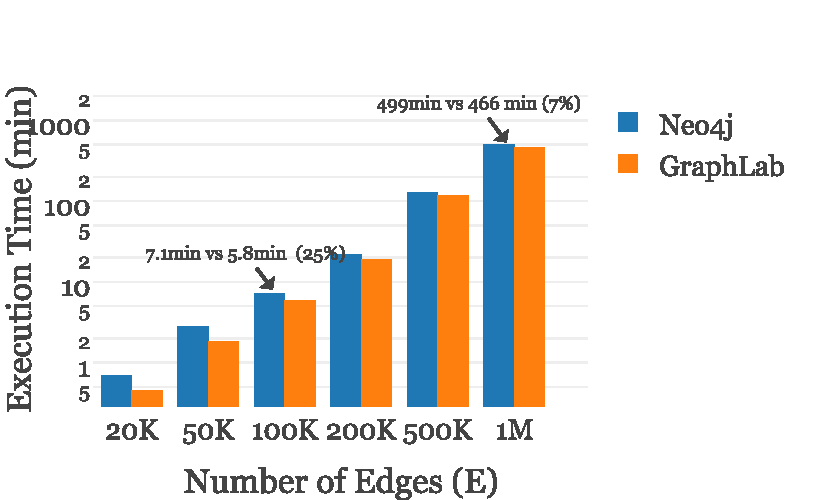
\includegraphics[scale=0.5]{Graphs/dense-edges.pdf}
			\caption{Dense datasets - Neo4j vs GraphLab\label{fig:dense-edges}}
		\end{minipage}
		\begin{minipage}{.5\textwidth}
			\centering
			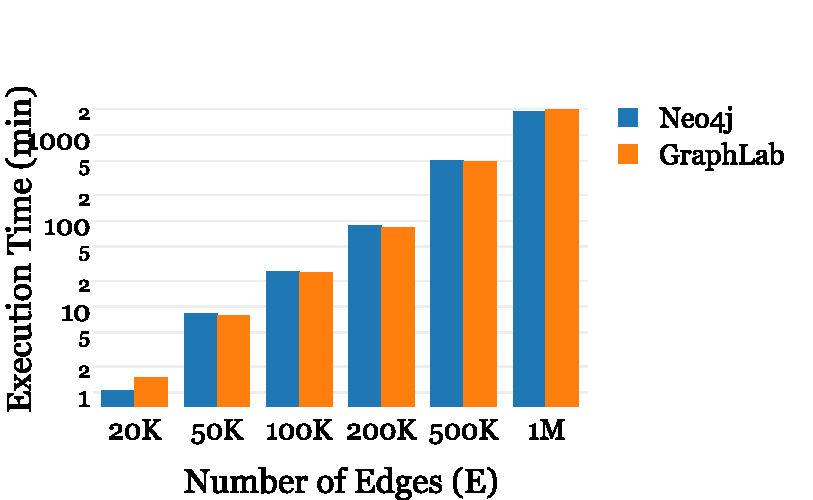
\includegraphics[scale=0.5]{Graphs/sparse-edges.pdf}
			\caption{Sparse datasets - Neo4j vs GraphLab\label{fig:sparse-edges}}
		\end{minipage}
	\end{figure}
	
	
	\begin{figure}
		\begin{minipage}{.5\textwidth}
			\centering
			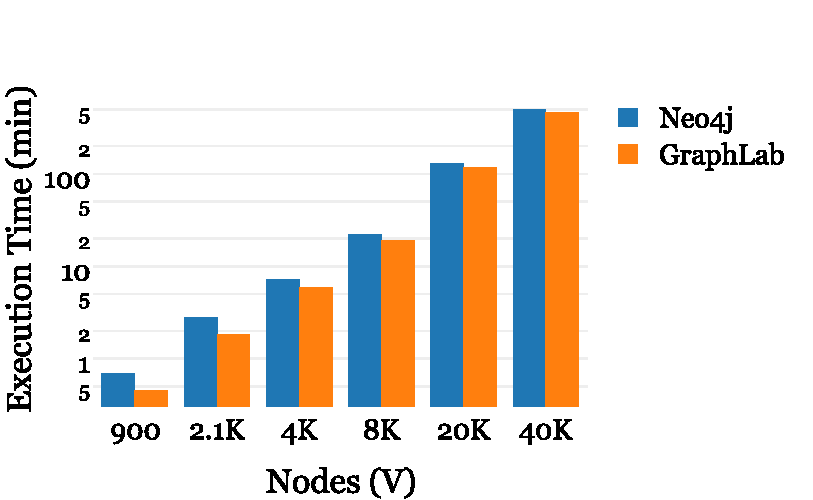
\includegraphics[scale=0.5]{Graphs/dense-nodes.pdf}
			\caption{Dense datasets - Neo4j vs GraphLab\label{fig:dense-nodes}}
		\end{minipage}
		\begin{minipage}{.5\textwidth}
			\centering
			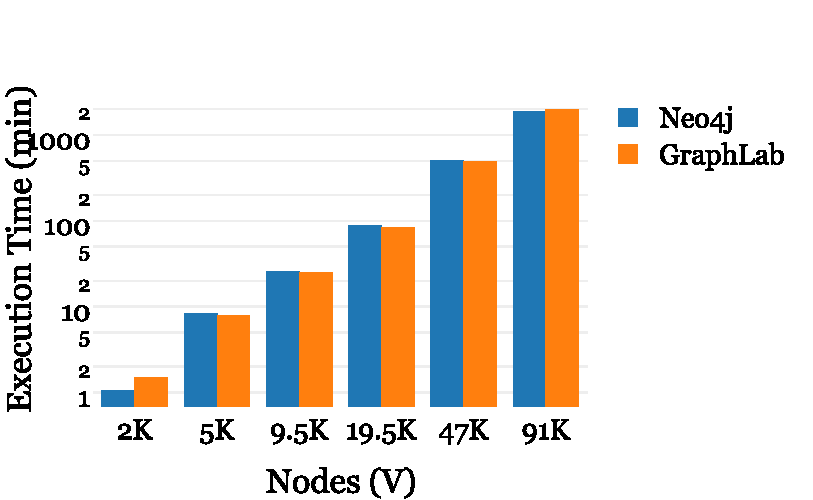
\includegraphics[scale=0.5]{Graphs/sparse-nodes.pdf}
			\caption{Sparse datasets - Neo4j vs GraphLab\label{fig:sparse-nodes}}
		\end{minipage}
	\end{figure}
	
	\begin{figure}
		\begin{minipage}{.5\textwidth}
			\centering
			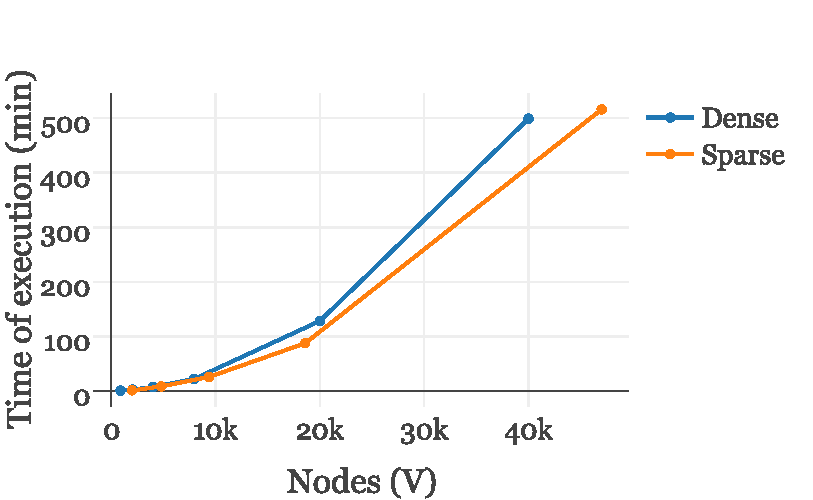
\includegraphics[scale=0.5]{Graphs/neo4j-sparse-dense.pdf}
			\caption{Neo4j - Dense vs Sparse datasets\label{fig:neo4j-sparse-dense}}
		\end{minipage}
		\begin{minipage}{.5\textwidth}
			\centering
			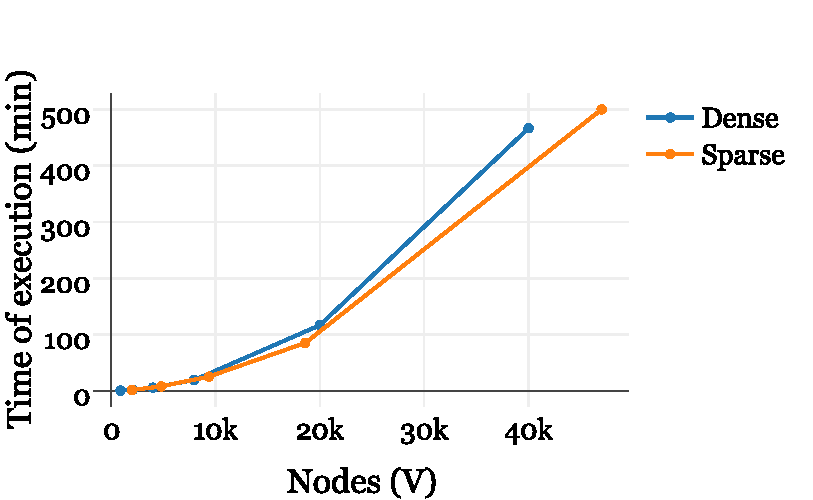
\includegraphics[scale=0.5]{Graphs/graphlab-sparse-dense.pdf}
			\caption{GraphLab - Dense vs Sparse datasets\label{fig:graphlab-sparse-dense}}
		\end{minipage}
	\end{figure}
	

\SubSection{Clustering on real world dataset: Facebook}
This section presents clustering performance of real world social network Facebook \cite{facebookdata} from Stanford Large Network Dataset Collection \cite{snap}.\\
\\
Facebook Dataset Details:
\begin{itemize}
	\item
	Nodes: 4039
	\item
	Edges: 88234
	\item
	Average clustering coefficient:	0.6055
	\item
	Number of triangles:	1612010
\end{itemize}
\noindent
Facebook Dataset Results:
\begin{itemize}
	\item
	Total number of clusters detected: 8
	\item
	List of clusters:\\
	Cluster-1 Nodes:1368\\
	Cluster-2 Nodes:770\\
	Cluster-3 Nodes:753\\
	Cluster-4 Nodes:590\\
	Cluster-5 Nodes:316\\
	Cluster-6 Nodes:211\\
	Cluster-7 Nodes:21\\
	Cluster-8 Nodes:10\\	
\end{itemize}
\begin{figure}[H]
	\centering
	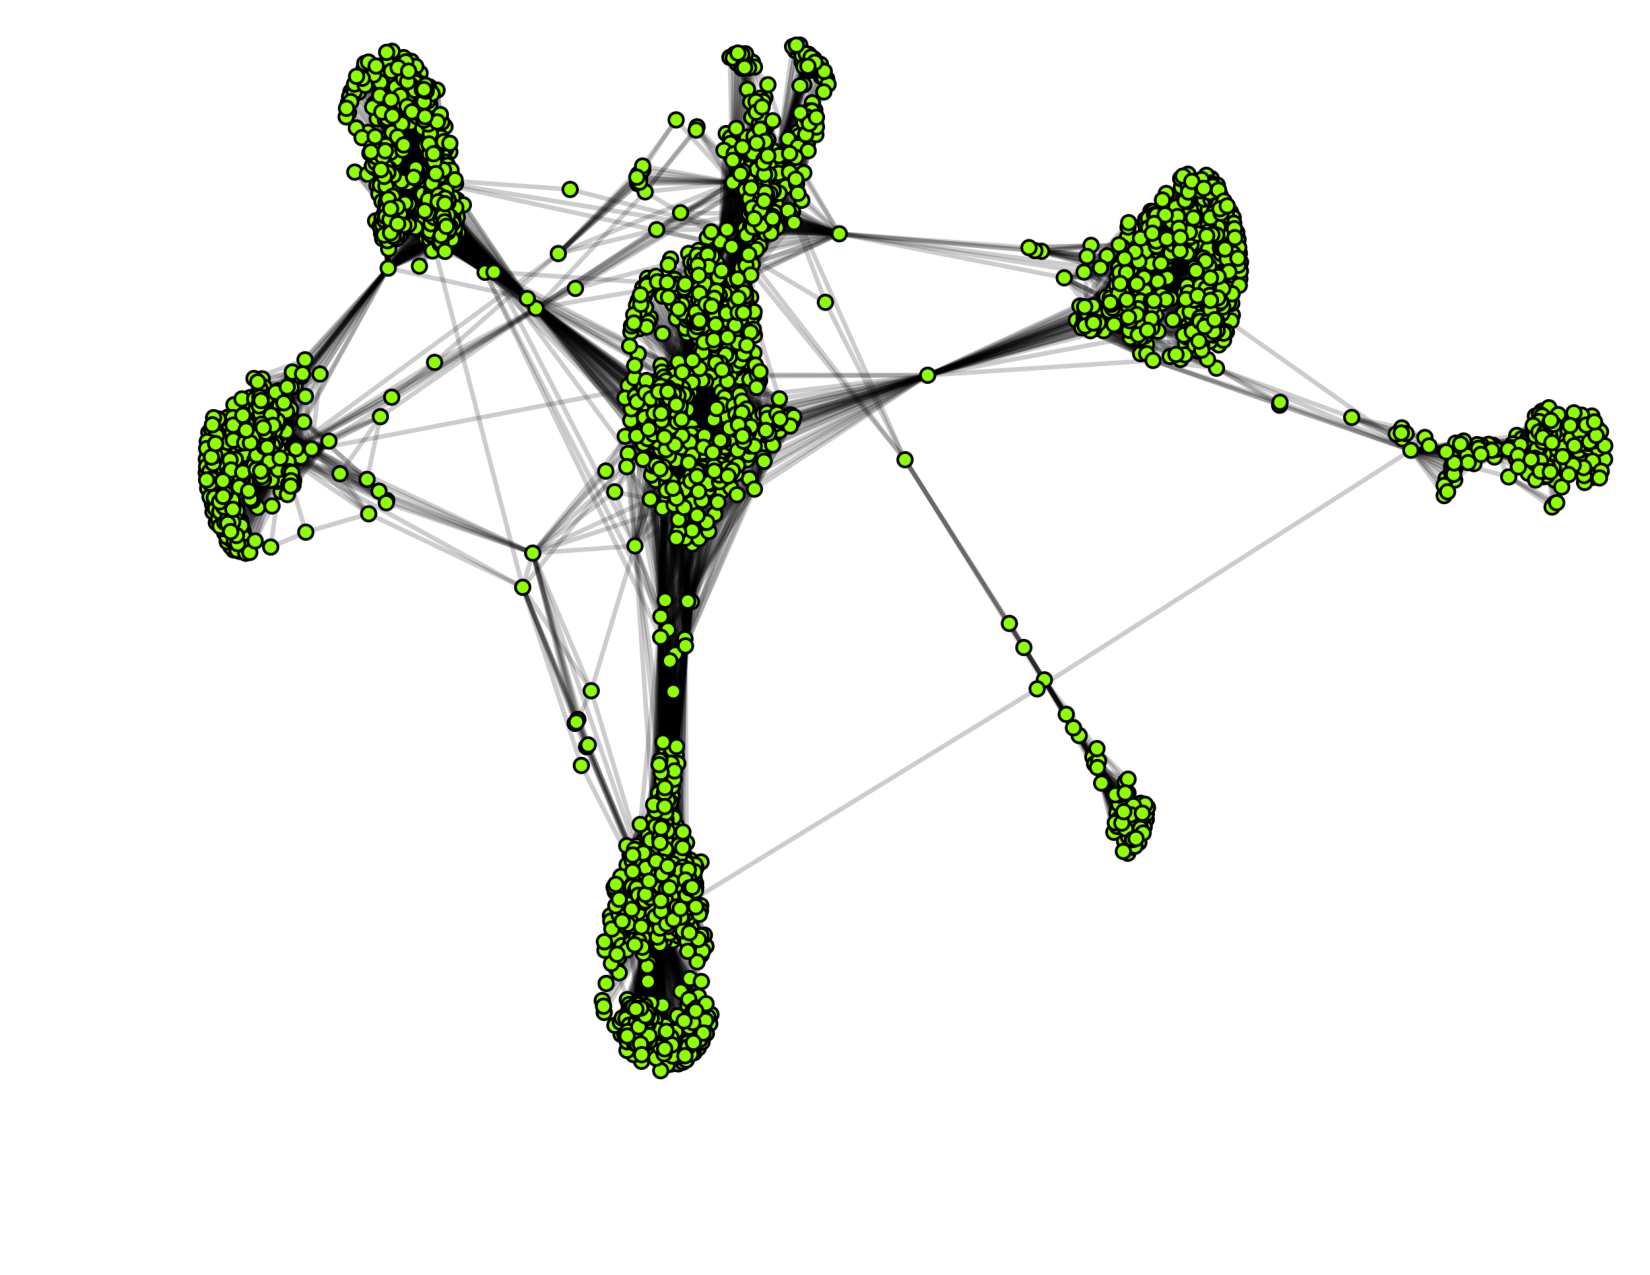
\includegraphics[scale=0.4, trim=0 0 20 0]{Images/before_facebook.pdf}
	\caption{Facebook Dataset - Before Clustering\label{fig:fb-before}}
\end{figure}
\begin{figure}[H]
	\centering
	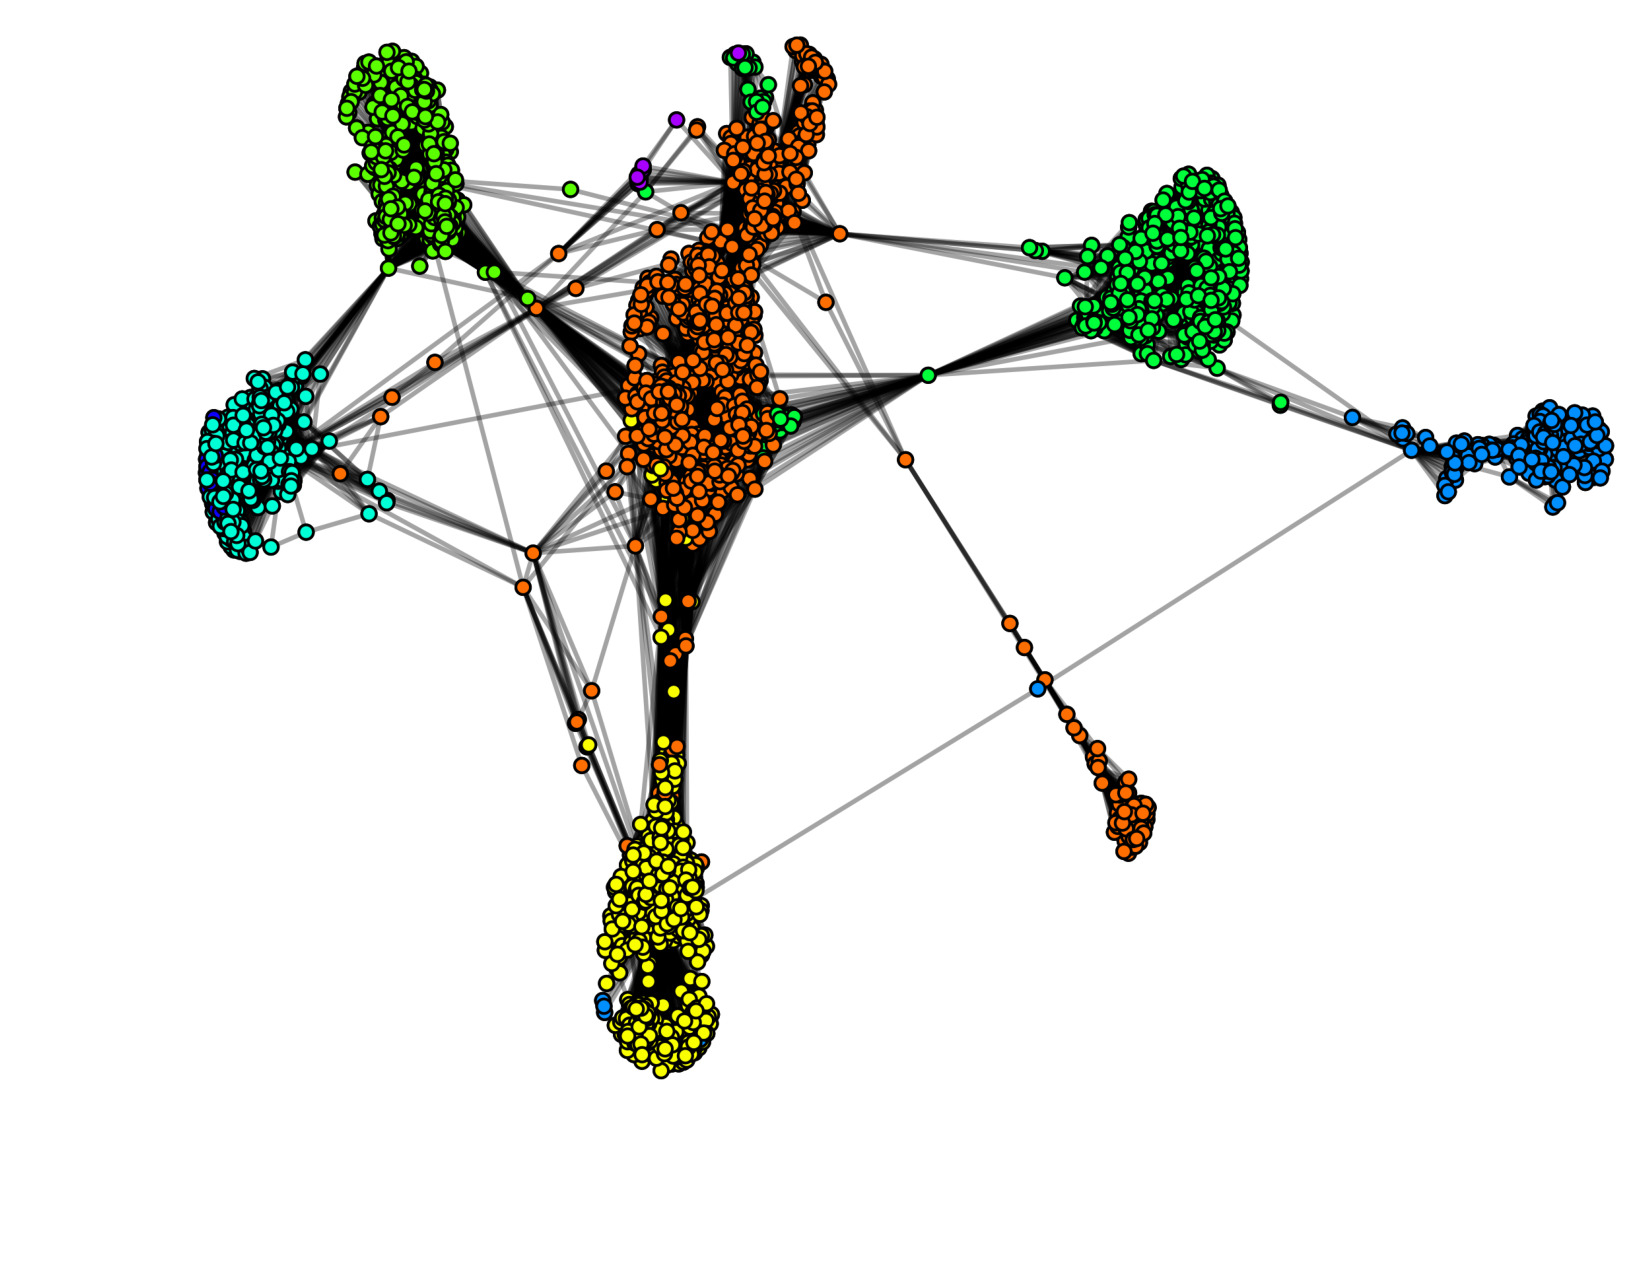
\includegraphics[scale=0.4, trim=0 0 20 0]{Images/after_facebook.pdf}
	\caption{Facebook Dataset - After Clustering\label{fig:fb-after}}
\end{figure}